\graphicspath{{./img/}} % path to graphics

\section*{\LARGE Введение}
\addcontentsline{toc}{section}{Введение}
Агентное моделирование - относительно новый метод моделирования.
Поначалу оно являлось преимущественно предметом теоретических дискуссий в
академических кругах, а начиная с 2000-х годов разработчики имитационных
моделей стали использовать его на практике.
Переход к агентному моделированию был вызван:

\begin{itemize}
	\item Желанием глубже изучить системы, которые сложно описать
		традиционными методами моделирования.
	\item Развитием технологии агентного моделирования
		(объектно-ориентированное моделирование, диаграммы состояний).
	\item Быстрому росту мощности процессоров и объема оперативной памяти
		компьютеров. Агентные модели более требовательны к ресурсам, чем
		модели системной динамики или дискретно-событийные модели.
\end{itemize}

Агентное моделирование предлагает разработчику моделей альтернативный
взгляд на поведение системы.

\clearpage

\section*{\LARGE Выполнение практической работы}
\addcontentsline{toc}{section}{Выполнение практической работы}

\section{Создание популяции агентов}
Начали с создания простой модели, которая продемонстрирует влияние
рекламы на начальные продажи продукта.\par
Люди в модели поначалу не будут пользоваться продуктом, но
потенциально могут быть в нем заинтересованы. Для начала создали
популяцию агентов, а потом задали то, как люди приобретают товар под
влиянием рекламы.\par
Чтобы добавить в модель потребителей, нам нужно создать новый тип
агента (потребитель) и затем создать популяцию агентов, которая будет состоять
из заданного количества агентов этого типа. Можно выполнить оба этих
действия с помощью удобного мастера создания агентов.\par

Открыли палитру \textbf{Агент}. Чтобы открыть другую палитру,
нужно перейти в панель Палитра и навести курсор мыши на вертикальную
панель навигации.\par
Перетащили элемент \textbf{Агент} из палитры \textbf{Агент}
на диаграмму Main.\par
Откроется мастер создания агентов \textbf{Новый агент}. Нужно создать
большое количество агентов одного типа, поэтому на первой странице
мастера выберали опцию \textbf{Популяция агентов}.\par

Типичная архитектура агентной модели в AnyLogic --- агент \textbf{Main},
на диаграмме которого заданы популяции агентов других типов.
В этом случае агент \textbf{Main} играет роль среды обитания
для других агентов. Среда задает тип пространства,
в котором живут агенты, расположение агентов в пространстве и сеть контактов
агентов, которая может использоваться при их общении друг с другом.\par

На данном этапе, создана простейшая агентной модели, и теперь можно
запустить ее и понаблюдать за поведением агентов
(Рисунок~\ref{fig:model:agent}).

\begin{image}
	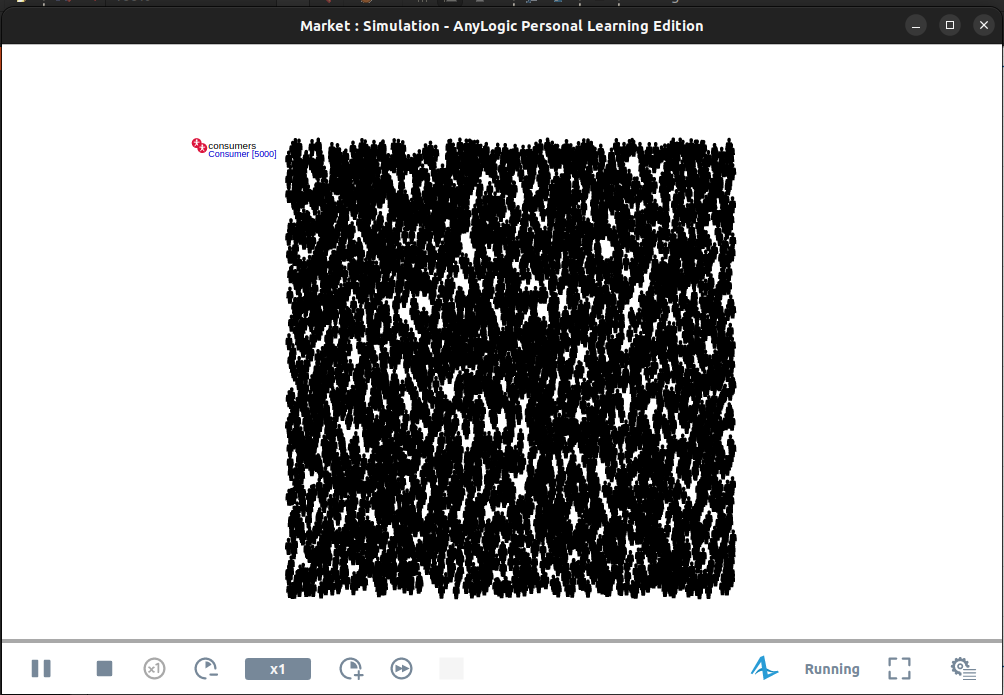
\includegraphics[width=0.9\textwidth]{Screenshot from 2023-03-27 20-00-54.png}
	\caption{Простейшая агентная модель}
	\label{fig:model:agent}
\end{image}

\section{Задание поведения потребителей}
На данном этапе задали поведение потребителей. Лучше всего задавать
поведение агента с помощью диаграммы состояний.\par
\textit{Диаграммы состояний} (карты состояний, стейтчарты) являются самым
удобным средством задания поведения агента. Диаграммы состояний
содержат состояния и переходы. Состояния диаграммы являются
взаимоисключающими, то есть в каждый момент времени агент может
находиться только в одном состоянии. Срабатывание перехода
приводит к смене состояния и активации новых переходов. Допускается
создание иерархических состояний, которые содержат внутри себя
другие состояния и переходы.\par
Задили поведение агента-потребителя как два последовательных
состояния:

\begin{itemize}
	\item PotentialUser --- находящийся в данном состоянии агент является
		потенциальным покупателем и может быть заинтересован в покупке.
	\item User --- потребитель, находящийся в этом состоянии,
		уже купил продукт.
\end{itemize}

Построение диаграммы состояний потребителя начинается с элемента
\textbf{Начало диаграммы состояний}.
Этот элемент определяет точку, инициирующую управление диаграммой, а
также задает имя этой диаграммы состояний.
Далее перетащили элемент \textbf{Состояние} из палитры
\textbf{Диаграмма состояний} в графический редактор и соедините
его с началом диаграммы. Нарисовали переход из состояния
\textbf{PotentialUser} в состояние \textbf{User}, чтобы промоделировать,
как человек приобретает продукт (и становится его потребителем).\par
Переход из одного состояния в другое может быть вызван событиями различных
типов. Для каждого типа приведен специальный значок, по которому легко
можно распознать тип перехода в диаграмме состояний.\par
Переход в создаваемой модели происходит с заданной интенсивностью.
Когда управление диаграммы состояний переходит в состояние
\textbf{PotentialUser}, происходит вычисление времени срабатывания перехода
согласно экспоненциальному распределению. Время до покупки продукта
для каждого отдельного потребителя будет отличаться, но в среднем
продукт будет приобретать 1\% потенциальных потребителей в день.\par
Теперь можно задать единицы модельного времени. Чтобы изменить
настройки модели, переключили из \textbf{Палитры} в панель \textbf{Проекты},
и затем щелкнули по элементу модели в дереве (самый верхний уровень дерева,
элемент Market). Перешили в панель \textbf{Свойства} и выберите дни в
качестве \textbf{Единиц модельного времени}.\par
\textit{Модельное время} --- это виртуальное (моделируемое) время
("внутреннее" время "движка" AnyLogic). Модельное время никак не
соотносится с реальным временем и часами на компьютере, хотя вы и
можете выполнять модель с привязкой модельного времени к
реальному.\par
Запустив модель, популяция агентов постепенно окрашивается в зеленый
цвет (изменение, к которому приводит эффект рекламы), пока каждый
потенциальный потребитель не купит продукт (Рисунок~\ref{fig:model:gedrag}).

\begin{image}
	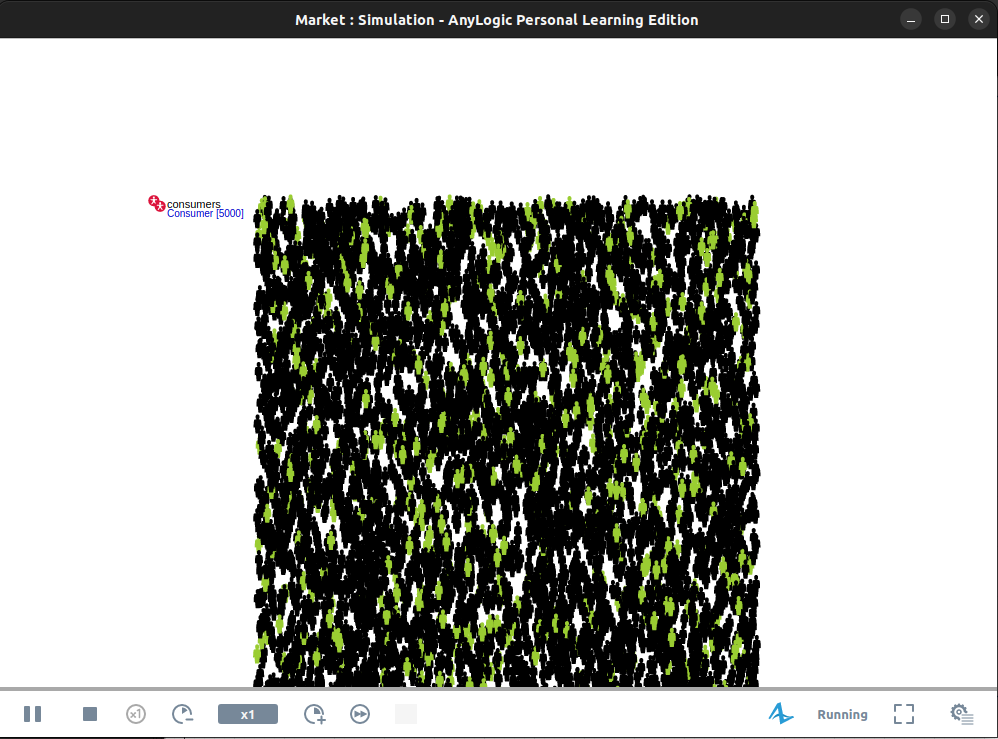
\includegraphics[width=0.9\textwidth]{Screenshot from 2023-03-28 09-28-37.png}
	\caption{Агентная модель с заданным поведением потребителей}
	\label{fig:model:gedrag}
\end{image}

\section[Добавление графика для визуализации результатов]
	{Добавление графика для визуализации результатов моделирования}
Чтобы знать, сколько людей приобрело продукт в определенный
момент времени. Задали функции, которые будут считать
количество потребителей и потенциальных потребителей продукта
соответственно, а затем добавили график, чтобы наблюдать за динамикой
изменения рынка.\par
Сначала задали функцию, которая будет считать количество потенциальных
потребителей. Чтобы добавить новую функцию подсчета статистики по
популяции агентов, открыли диаграмму агента \textbf{Main}, выделили популяцию
агентов \textit{consumers} и перейшли в раздел
свойств \textbf{Статистика}. И добавили функции \textit{NPotential} и
\textit{NUser} с условиями соответственно
\texttt{item.inState(Consumer.PotentialUser)}
и \texttt{item.inState(Consumer.User)}\par
Затем добавили график для визуального отображения статистики,
собираемой заданными только что функциями, и понабли за динамикой
внедрения нового продукта на рынок.\par
Указали, какие данные будет отображать график. Воспользовавшись теми
самыми функциями статистики \textit{NUser} и \textit{NPotential},
которые были созданы ранее для популяции consumers.\par
Запустив модель, теперь можно понаблюдать за моделируемым процессом с помощью
добавленной диаграммы (Рисунок~\ref{fig:graphic}).

\begin{image}
	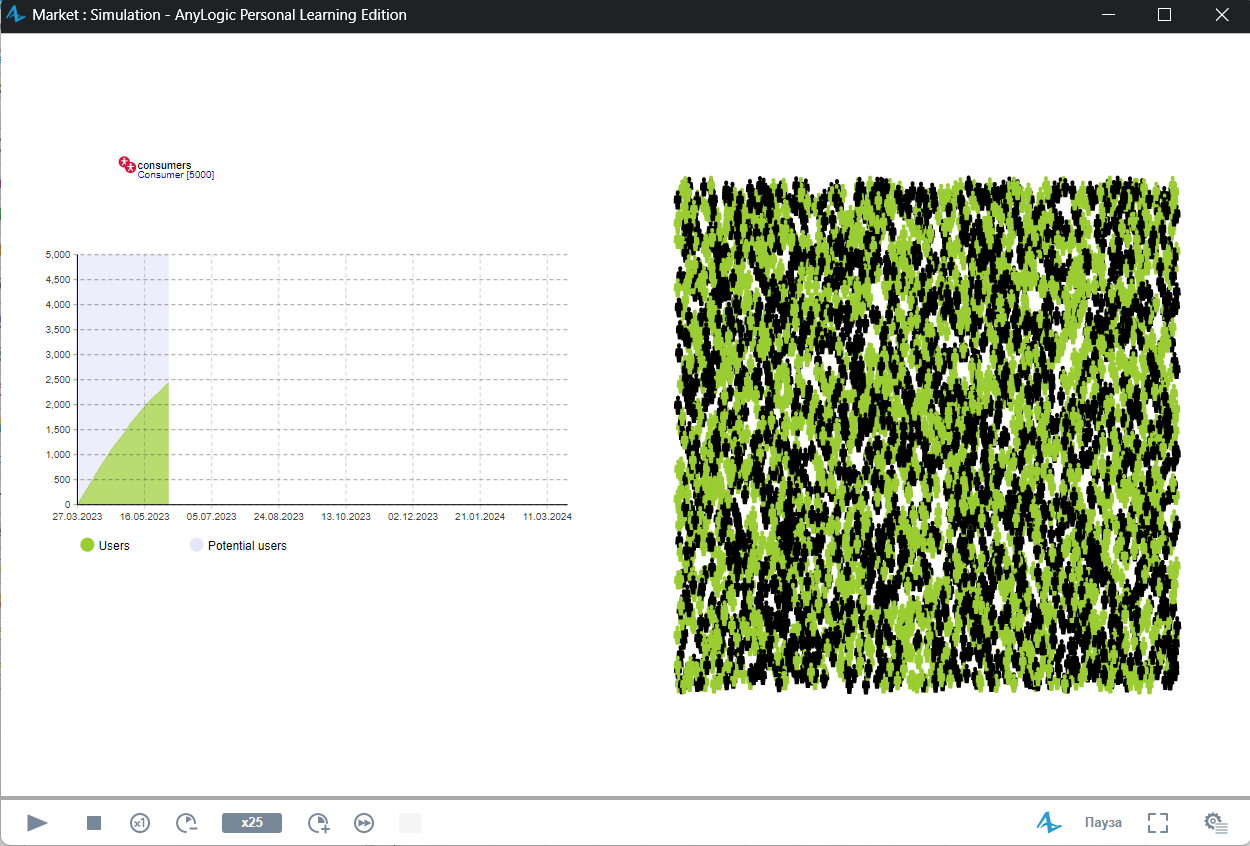
\includegraphics[width=0.9\textwidth]{2023-03-28_17-04-51}
	\caption{Запущеная модель с графиком}
	\label{fig:graphic}
\end{image}

\section{Добавление эффекта рекомендаций}
На данном этапе промоделировали эффект, который оказывают на потенциальных
потребителей положительные отзывы о продукте его владельцев.

\begin{itemize}
	\item В модели каждый человек в течение дня будет в среднем
		общаться с одним своим знакомым.
	\item Во время общения друг с другом владельцы продукта могут повлиять на
		потенциальных потребителей. Задали вероятность приобретения
		продукта потенциальным потребителем под воздействием общения с
		помощью параметра \texttt{AdoptionFraction = 0.01}.
\end{itemize}

Для начала добавили два новых параметра: \texttt{ContactRate} (определяет
интенсивность контактов) и \texttt{AdoptionFraction} (вероятность приобретения
продукта в результате общения с пользователем этого продукта).\par
В модели сообщения будут посылать только те агенты, которые находятся
в состоянии \texttt{User}. Лучшим способом задать действие,
которое агент выполняет, не выходя из текущего состояния,
является добавление внутреннего перехода.\par
Создав циклический переход в состоянии \textit{User}. Каждый раз, когда
срабатывает этот переход, вызываемая функция \texttt{sendToRandom("Buy")}
моделирует отправку этим потребителем сообщения \texttt{“Buy”} случайно
выбранному агенту. Если агент, который получает сообщение, является
потенциальным потребителем (то есть находится в состоянии
\textit{PotentialUser}), то текущим состоянием агента-получателя станет
состояние \textit{User} (согласно еще одному переходу,
который мы нарисуем сейчас).\par
Насыщение рынка теперь будет происходить быстрее, а график покажет
известную S-образную кривую выхода нового продукта на рынок
(Рисунок~\ref{fig:recommend}).

\begin{image}
	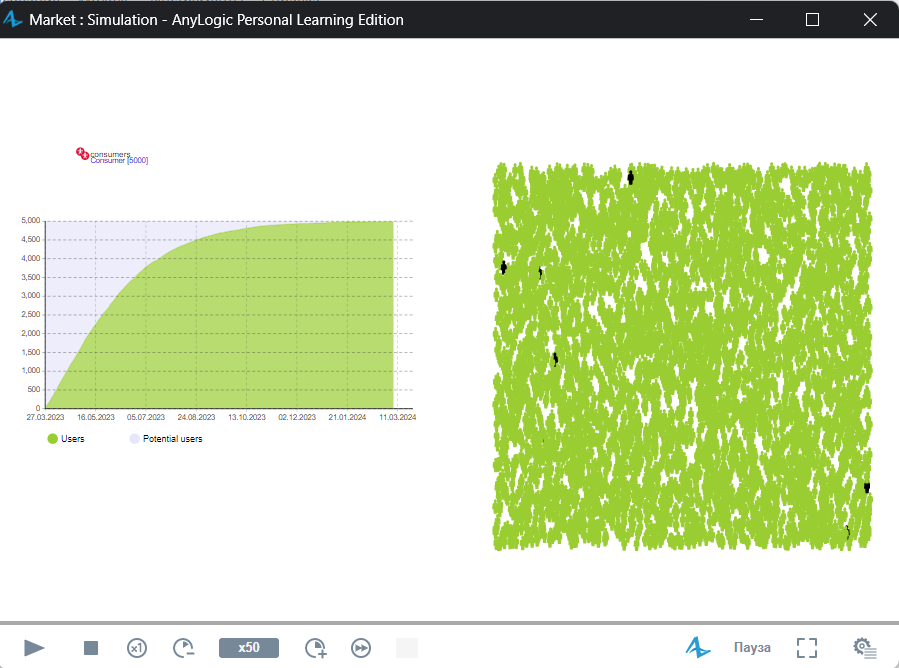
\includegraphics[width=0.9\textwidth]{2023-03-28_17-15-52}
	\caption{S-образная кривая выхода нового продукта на рынок}
	\label{fig:recommend}
\end{image}

\section{Учет повторных продаж продукта}
Допустив, что у рассматриваемого продукта ограниченный срок годности
(или срок эксплуатации), равный шести месяцам.
Когда потребитель больше не cможет пользоваться продуктом, ему понадобится
замена продукта. Смоделировали повторные покупки, предположив, что по
истечении срока годности товара потребители вновь становятся
потенциальными потребителями (то есть, агенты переходят из состояния
\textit{User} обратно в состояние \textit{PotentialUser}).\par
Итак, учтя в модели ограничение срока службы товара, приводящее к
повторным покупкам товара потребителями, график вышел таким, как
показано на рисунке~\ref{fig:repeat:sales}.

\begin{image}
	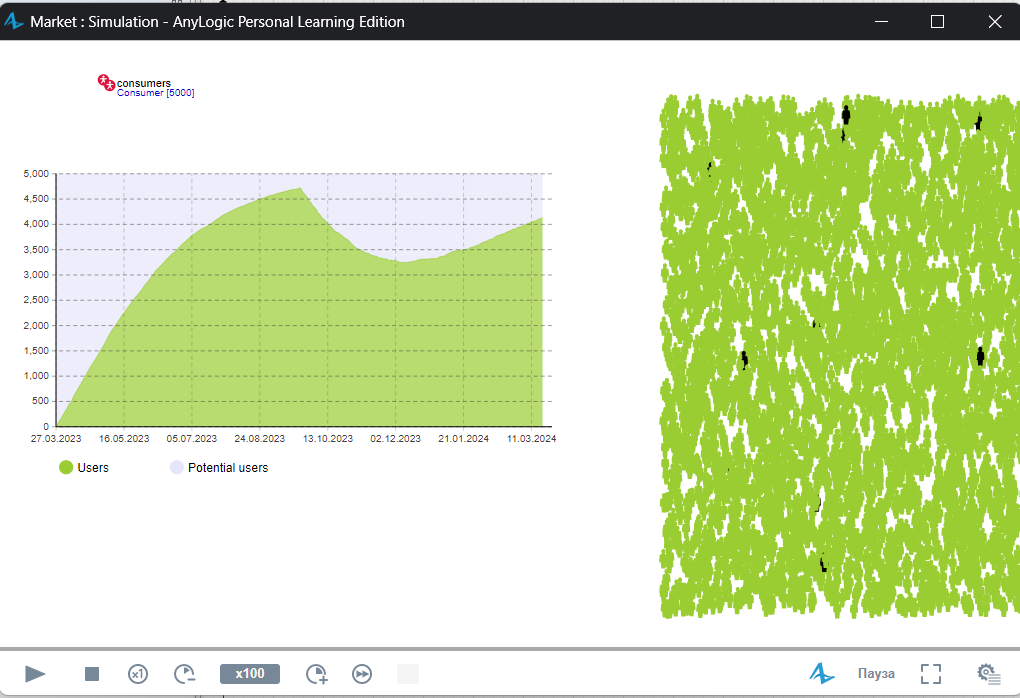
\includegraphics[width=0.9\textwidth]{2023-03-28_17-20-05}
	\caption{График с повторными продажами}
	\label{fig:repeat:sales}
\end{image}

Сама модель показана на рисунке~\ref{fig:repeat:sales:model}.

\begin{image}
	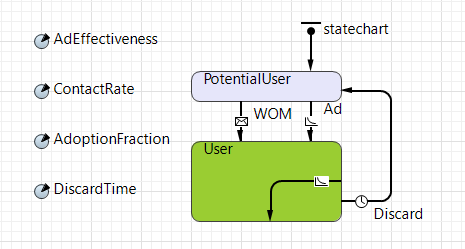
\includegraphics[width=0.9\textwidth]{2023-03-28_17-20-26}
	\caption{Модель с повторными продажами}
	\label{fig:repeat:sales:model}
\end{image}

\section{Учет времени доставки продукта}
В текущей модели предполагается, что продукт всегда есть в наличии, и
поэтому переход из состояния \textit{PotentialUser} в состояние
\textit{User} происходит моментально. На данном этапе усовершенствовали
модель, добавив у потребителя еще одно состояние, которое будет
соответствовать времени, проходящему с момента принятия решения о покупке
продукта до момента появления товара в продаже и доставки его покупателю.\par
Добавили новое состояние в середину диаграммы состояний потребителя
и назвали его \textit{WantsToBuy} («хочет купить»). Потребители в этом
состоянии решили купить продукт, но продукт пока еще не приобрели.\par
Выделили переходы \textit{WOM} и \textit{Ad} и переместите их конечные
точки выше, затем отсоедините переход \textit{Discard} от состояния
\textit{PotentialUser}.\par
Запустив модель, люди, ожидающие доставки товара, будут отображаться
на графике и на анимации желтым цветом, как
показано на рисунке~\ref{fig:delivery:time}.

\begin{image}
	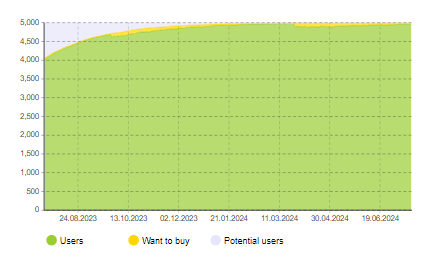
\includegraphics[width=0.9\textwidth]{2023-03-28_17-33-21}
	\caption{График времени доставки продукта}
	\label{fig:delivery:time}.
\end{image}

Сама модель показана на рисунке~\ref{fig:delivery:time:model}.

\begin{image}
	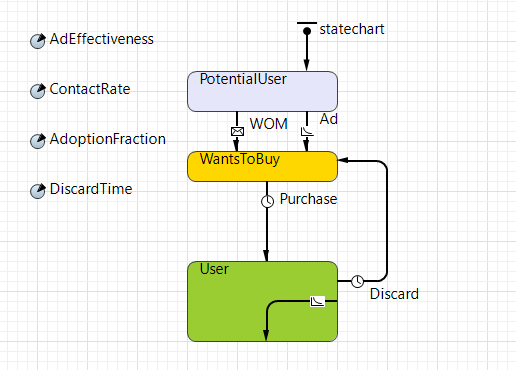
\includegraphics[width=0.9\textwidth]{2023-03-28_17-31-28}
	\caption{Модель с повторными продажами}
	\label{fig:delivery:time:model}
\end{image}

\section{Моделирование отказов от покупки товара}
Теперь можно учесть тот факт, что время, которое потребители согласны
потратить на ожидание доставки товара, конечно. Если время доставки превысит
предельно допустимое время ожидания, потребитель откажется от покупки.\par
Начили с того, что добавили на диаграмму \textit{Main} два параметра,
задающих максимальное время доставки товара (25 дней) и максимальное
время ожидания доставки (7 дней) соответственно.\par
Таким образом, доставка товара может длиться от одного до 25 дней, в среднем
же доставка занимает два дня. Надо изменить значение времени доставки с
фиксированного периода, равного двум дням, на стохастическое выражение,
которое использует вышеуказанный диапазон значений.\par
Далее выбрали треугольное распределение вероятности для задания времени
ожидания, как самое подходящее.\par
Задали максимальное время ожидания с помощью треугольного
распределения со средним значением, равным параметру \textit{MaxWaitingTime}
(т.е., одной неделе), и отклонением от этого значения, равным 15 процентам.
Использовали параметр, а не просто указываем соответствующее значение
времени для того, чтобы впоследствии иметь возможность варьировать это
значение динамически и наблюдать эффект от производимых изменений прямо
по ходу моделирования. Одним из способов создания интерактивной модели
является добавление элементов управления и связывание их с варьируемыми
параметрами.\par
Добавили бегунок --- элемент управления, который позволяет выбирать
числовое значение из определенного интервала. Бегунок часто используется для
того, чтобы изменять значения численных переменных и параметров.\par
Полученный график показан на рисунке~\ref{fig:refusals}.

\begin{image}
	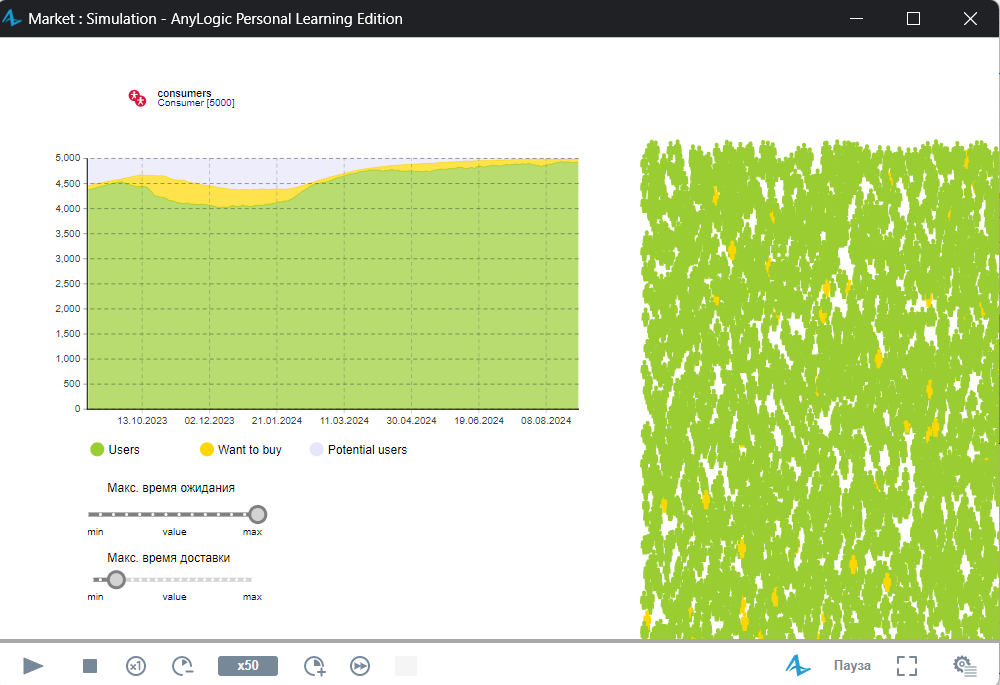
\includegraphics[width=0.8\textwidth]{2023-03-28_17-48-54}
	\caption{График с добавлением отказов от покупок}
	\label{fig:refusals}.
\end{image}


\section{Сравнение прогонов модели}
Эта фаза не реализована, так как для нее требуется pro-версия приложения.

\clearpage

\section*{\LARGE Вывод}
\addcontentsline{toc}{section}{Вывод}
В данной практической работе была создана агентная модель потребительского
рынка. В ходе работы были созданы популяция агентов, задано поведение
потребителей. Добавлены графики с эффектом рекомендаций и учетем повторных
продаж и времени доставки.

